\documentclass[a4paper]{article}
\usepackage{pdp}
\usepackage{listings}
\usepackage{xcolor}
\usepackage{tcolorbox}
\usepackage{enumitem}
\usepackage{amsmath}
\usepackage{minted}
\usepackage{tocloft}
\usepackage{tikz}
\usepackage{graphicx}
\usepackage{caption}

\tcbuselibrary{skins, breakable}
\newtcolorbox{besoinbox}{
    colback=white,
    colframe=blue!75!black,
    fonttitle=\bfseries,
    coltitle=black,
    colbacktitle=blue!75!black,
    enhanced,
    attach boxed title to top left={yshift=-3mm, xshift=5mm},
    boxrule=0.5pt,
    breakable,
    arc=4pt,
    left=6pt,
    right=6pt,
    top=6pt,
    bottom=6pt
}

\lstset{
    language=Java,
    basicstyle=\ttfamily\footnotesize,
    numbers=left,
    numberstyle=\tiny,
    stepnumber=1,
    numbersep=5pt,
    backgroundcolor=\color{white},
    showspaces=false,
    showstringspaces=false,
    showtabs=false,
    frame=single,
    rulecolor=\color{black},
    tabsize=2,
    captionpos=b,
    breaklines=true,
    breakatwhitespace=false,
    keywordstyle=\color{blue},
    commentstyle=\color{green},
    stringstyle=\color{red}
}

\title{Scrabble -- Java}
\author{CODOGNAN Thomas, KAHLOUL Aïssa, BETTCHER Léonard, BLOTHIAUX Yanis, RAZE Erwan}

\begin{document}
\maketitle

\section*{Introduction}
\addcontentsline{toc}{section}{Introduction}
\hangindent=0.8mm
\hangafter=1
Ce rapport préliminaire expose les fondations théoriques et architecturales du projet Scrabble en Java. Nous présentons l'historique du jeu, sa nature combinatoire, les défis algorithmiques qu'il pose, puis détaillons nos choix d'architecture et de structures de données.

\section{Historique et Nature du Sujet}

\subsection{Historique du sujet}
\hangindent=0.8mm
\hangafter=1
En 1931, l'architecte Alfred Mosher Butts crée un jeu combinant chance et réflexion. Après avoir analysé la fréquence des lettres dans le New York Times, il conçoit le système de points spécifique aux jetons. D’abord nommé Lexiko, puis Criss-Cross Words, le jeu est racheté en 1948 par James Brunot qui le baptise Scrabble. Le succès explose dans les années 1950 grâce à Jack Straus (président de Macy's) qui en lance la commercialisation massive. 
\vspace{1\baselineskip}

\subsection{Nature et enjeux du jeu}
\hangindent=0.8mm
\hangafter=1
Le Scrabble est un jeu de lettres à \textbf{information imparfaite} (les tirages adverses sont cachés) et \textbf{stochastique} (dû au hasard de la pioche). L'objectif est de maximiser un score sur une grille (standard de $15 \times 15$ ou Super Scrabble de $21 \times 21$) en plaçant des mots d'un dictionnaire de référence.

\hangindent=0.8mm
\hangafter=1
Le jeu repose sur trois piliers :

\hangindent=1.5cm
\hangafter=1
\textbf{1. Logique spatiale :} Respect de la connexité (tout mot doit être rattaché aux lettres déjà posées et toutes les lettres posées se touchent entre elles) et de l'orthogonalité (validité de tous les mots formés par collision).

\vspace{1\baselineskip}
\hangindent=1.5cm
\hangafter=1
\textbf{2. Logique mathématique :} Calcul dynamique des points incluant la valeur des lettres et les multiplicateurs de cases (lettre/mot compte double/triple), appliqués dans l'ordre (lettres puis mots), ainsi que le bonus de 50 points (\textit{Scrabble}) pour l'usage des 7 lettres du chevalet.

\vspace{1\baselineskip}
\hangindent=1.5cm
\hangafter=1
\textbf{3. Logique linguistique :} Arbitrage instantané de la validité des mots selon le lexique choisi.

\subsubsection*{Déroulement et règles de jeu}
\hangindent=0.8mm
\hangafter=1
\textbf{Début de partie :} Le premier joueur doit placer un mot de deux lettres ou plus couvrant la case centrale, doublant ainsi le score de ce mot.

\hangindent=1.5cm
\hangafter=1
\textit{Exemple :} Si le premier joueur place le mot \og AXE \fg{} avec le \og X \fg{} sur la case centrale (H8), le score du mot ($9 + 8 + 1 = 18$) est doublé pour un total de 36 points.

\vspace{1\baselineskip}
\hangindent=0.8mm
\hangafter=1
\textbf{Actions du joueur :} À chaque tour, le joueur peut poser un mot, échanger des jetons avec le sac (si celui-ci contient au moins 7 lettres) ou passer son tour.

\hangindent=1.5cm
\hangafter=1
\textit{Exemple de collision :} Si le mot \og FEU \fg{} est déjà sur le plateau, un joueur peut placer \og R \fg{} au-dessus du \og E \fg{} pour former \og RE \fg{} verticalement tout en posant \og RATS \fg{} horizontalement.

\vspace{1\baselineskip}
\hangindent=0.8mm
\hangafter=1
\textbf{Notation des coups :} Les coups sont notés par leurs coordonnées de départ suivies du mot et du score (ex: \texttt{H8 - VERSION - 34 pts}).

\hangindent=1.5cm
\hangafter=1
\textit{Exemple :} La notation \og \texttt{8H} \fg{} indique un mot horizontal commençant à la ligne 8, colonne H, tandis que \og \texttt{H8} \fg{} indique un mot vertical commençant à la colonne H, ligne 8.

\vspace{1\baselineskip}
\hangindent=0.8mm
\hangafter=1
\textbf{Fin de partie et victoire :} La partie s'achève quand le sac est vide et qu'un joueur a épuisé son chevalet, ou après trois tours sans score (blocage). Le vainqueur est celui ayant le score le plus élevé après déduction de la valeur des lettres restantes sur les chevalets. Un match nul est possible si les scores finaux sont identiques.

\hangindent=1.5cm
\hangafter=1
\textit{Exemple de calcul final :} Si le joueur A finit avec 300 points et que le joueur B possède encore un \og W \fg{} (10 pts) et un \og X \fg{} (10 pts) sur son chevalet, le score de B sera réduit de 20 points, et ces 20 points seront ajoutés au score de A.

\subsection{Complexité du jeu}
\hangindent=0.8mm
\hangafter=1
Il est crucial de distinguer la complexité intrinsèque du jeu de celle des algorithmes utilisés.

\hangindent=0.8mm
\hangafter=1
\textbf{Espace d'état :} Le nombre de positions légales sur un plateau de $15 \times 15$ est estimé à environ $10^{30}$. Bien que moindre que celui des échecs, l'incertitude sur les jetons restants complexifie la recherche.

\hangindent=1.5cm
\hangafter=1
\textit{Détail du calcul combinatoire :} Pour un chevalet de 7 lettres et un dictionnaire type ODS (380\,000 mots), le nombre de placements théoriques au premier tour est le produit des arrangements $P(7, n)$ par les orientations et positions sur l'étoile centrale.

\vspace{1\baselineskip}
\hangindent=0.8mm
\hangafter=1
\textbf{Heuristiques et incertitude :} Le score immédiat n'est pas le seul facteur. Une stratégie gagnante doit évaluer la \og qualité du reliquat \fg{} (garder des lettres polyvalentes comme les voyelles ou le \og S \fg{}) et l'obstruction (ne pas ouvrir de cases bonus pour l'adversaire).

\subsection{Problématique algorithmique}
\hangindent=0.8mm
\hangafter=1
La difficulté majeure est l'explosion combinatoire. Le moteur doit :

\hangindent=1.5cm
\hangafter=1
\textbf{1. Rechercher exhaustivement} tous les coups légaux en un temps imperceptible.

\vspace{1\baselineskip}
\hangindent=1.5cm
\hangafter=1
\textbf{2. Simuler une IA} capable de prendre des décisions non-déterministes en gérant l'état futur du plateau et l'accessibilité aux bonus après le coup, afin de permettre la création de parties joueurs/intelligences artificielles.

\subsection{Existant}
\hangindent=0.8mm
\hangafter=1
L'état de l'art repose sur des travaux académiques et des logiciels éprouvés :

\hangindent=1.5cm
\hangafter=1
\textbf{1. Littérature scientifique :} L'algorithme de référence pour la génération rapide de coups est celui de Steven Gordon (GADDAG) ou le travail d'Appel et Guy (DAWG). Ces structures minimisent l'espace mémoire tout en maximisant la vitesse de parcours du dictionnaire.

\vspace{1\baselineskip}
\hangindent=1.5cm
\hangafter=1
\textbf{2. Logiciels de référence :} \textbf{Quackle} est le standard pour l'analyse stratégique. Il utilise des simulations de Monte-Carlo pour comparer les coups en fonction de l'espérance de gain sur les tours suivants.

\vspace{1\baselineskip}
\hangindent=1.5cm
\hangafter=1
\textbf{3. Plateformes :} L'ISC (\textit{Internet Scrabble Club}) sert de référence pour la pratique compétitive ou classique, garantissant une application stricte des règles internationales.

\section{Algorithmes et Structures de Données}
\hangindent=0.8mm
\hangafter=1
L'implémentation d'un joueur artificiel performant au Scrabble repose sur la résolution de deux problèmes distincts : la génération efficace de tous les coups légaux et la sélection du meilleur coup parmi ceux-ci. Cette section détaille les choix algorithmiques retenus pour répondre à ces besoins.

\subsection{Modélisation du problème}
\hangindent=0.8mm
\hangafter=1
Contrairement aux Échecs ou au Go, qui sont des jeux à information parfaite et déterministes, le Scrabble est un jeu à information imparfaite, on ne connait pas lettres de l'adversaire et le tirage des lettres repose sur le hasard.

\hangindent=0.8mm
\hangafter=1
Une approche gloutonne, qui consisterait à jouer systématiquement le coup rapportant le plus de points à l'instant $t$, est sous-optimale. Elle néglige deux facteurs cruciaux :

\hangindent=1.5cm
\hangafter=1
\textbf{1. Le reliquat (Rack Leave) :} La qualité des lettres conservées pour le tour suivant.

\vspace{1\baselineskip}
\hangindent=1.5cm
\hangafter=1
\textbf{2. L'ouverture du plateau :} Le risque d'offrir une case "Mot Compte Triple" à l'adversaire.

\subsection{L'Algorithme Minimax}
\hangindent=0.8mm
\hangafter=1
L'algorithme Minimax est la base de la décision dans les jeux à somme nulle. Il parcourt l'arbre de jeu jusqu'à une profondeur $d$ donnée.

\begin{figure}[H]
    \centering
    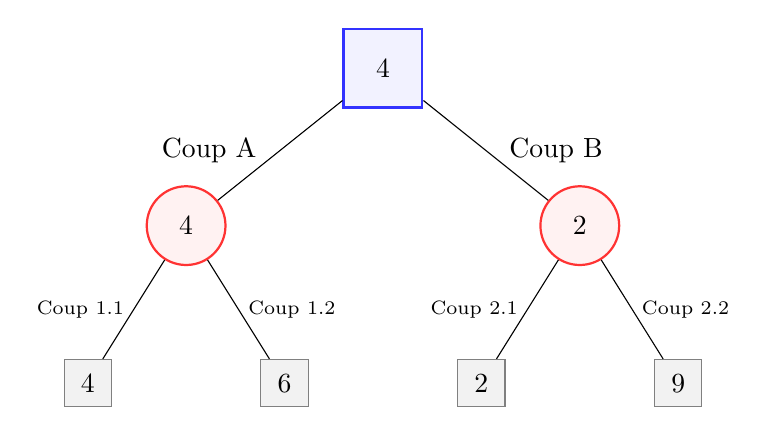
\begin{tikzpicture}[
        level 1/.style={sibling distance=5cm},
        level 2/.style={sibling distance=2.5cm},
        level distance=2cm,
        % Styles des nœuds
        maxnode/.style={rectangle, draw=blue!80, thick, minimum size=10mm, fill=blue!5, text centered},
        minnode/.style={circle, draw=red!80, thick, minimum size=10mm, fill=red!5, text centered},
        leaf/.style={rectangle, draw=gray, thin, minimum size=6mm, fill=gray!10},
        % Style des flèches de remontée de valeur
        valueprop/.style={->, dashed, thick, color=orange}
    ]

    % Racine (MAX)
    \node[maxnode] (root) {4}
        % Branche Gauche (MIN)
        child { 
            node[minnode] {4} 
            child { node[leaf] {4} edge from parent node[left, font=\scriptsize] {Coup 1.1} }
            child { node[leaf] {6} edge from parent node[right, font=\scriptsize] {Coup 1.2} }
            edge from parent node[left, xshift=-5pt] {Coup A}
        }
        % Branche Droite (MIN)
        child { 
            node[minnode] {2}
            child { node[leaf] {2} edge from parent node[left, font=\scriptsize] {Coup 2.1} }
            child { node[leaf] {9} edge from parent node[right, font=\scriptsize] {Coup 2.2} }
            edge from parent node[right, xshift=5pt] {Coup B}
        };

    \end{tikzpicture}
    \caption{Exemple de déroulement d'un arbre Minimax}
    \label{fig:minimax_tree}
\end{figure}

\subsubsection*{Fonctionnement}
\hangindent=0.8mm
\hangafter=1
L'algorithme alterne entre deux types de nœuds :

\hangindent=1.5cm
\hangafter=1
\textbf{1. Nœuds MAX :} Cherche à maximiser le score final.

\vspace{1\baselineskip}
\hangindent=1.5cm
\hangafter=1
\textbf{2. Nœuds MIN :} Cherche à minimiser le score.

\hangindent=0.8mm
\hangafter=1
L'application stricte de Minimax au Scrabble pose un problème de modélisation. Minimax suppose que l'adversaire jouera toujours le coup optimal pour nous contrer. Or, pour déterminer ce coup optimal, l'algorithme doit connaître les lettres de l'adversaire. Dans une simulation Minimax, nous devrions supposer le pire cas : l'adversaire possède exactement les lettres nécessaires pour réfuter notre coup (ex: un "Z" pour atteindre un mot compte triple ouvert). Cette approche rend l'IA excessivement défensive et inadaptée à la réalité probabiliste du tirage.

\begin{besoinbox}
\captionof{lstlisting}{Pseudo-code de l'algorithme Minimax}
\label{lst:minimax_algo}
\begin{minted}[frame=lines, framesep=2mm, baselinestretch=1.2, fontsize=\footnotesize, linenos]{text}
Fonction Minimax(état, profondeur, est_joueur_max):
    // Cas de base : feuille de l'arbre ou profondeur atteinte
    SI profondeur == 0 OU partie_terminée(état) ALORS
        RETOURNER evaluer(état)

    SI est_joueur_max ALORS
        // Tour de l'IA (Cherche à maximiser son score)
        meilleure_valeur = -INFINI
        POUR CHAQUE coup DANS generer_coups_possibles(état) FAIRE
            nouvel_état = jouer_coup(état, coup)
            valeur = Minimax(nouvel_état, profondeur - 1, FAUX)
            meilleure_valeur = MAX(meilleure_valeur, valeur)
        RETOURNER meilleure_valeur

    SINON
        // Tour de l'adversaire (Cherche à minimiser notre gain)
        pire_valeur = +INFINI
        POUR CHAQUE coup DANS generer_coups_possibles(état) FAIRE
            nouvel_état = jouer_coup(état, coup)
            valeur = Minimax(nouvel_état, profondeur - 1, VRAI)
            pire_valeur = MIN(pire_valeur, valeur)
        RETOURNER pire_valeur
\end{minted}
\end{besoinbox}

\subsection{L'Algorithme Expectiminimax}
\hangindent=0.8mm
\hangafter=1
Pour intégrer la dimension aléatoire du tirage de lettres, nous utilisons l'algorithme \textbf{Expectiminimax}. C'est une variation du Minimax qui introduit un troisième type de nœud : les \textbf{Nœuds de Hasard}.

\vspace{1\baselineskip}
\hangindent=0.8mm
\hangafter=1
L'arbre de décision se décompose désormais en trois niveaux par tour de jeu :

\hangindent=1.5cm
\hangafter=1
\textbf{1. Nœud MAX :} L'IA choisit un coup parmi les coups possibles générés.

\vspace{1\baselineskip}
\hangindent=1.5cm
\hangafter=1
\textbf{2. Nœud CHANCE :} Ce nœud représente l'incertitude sur les lettres de l'adversaire. Il possède une branche pour chaque tirage possible, pondérée par sa probabilité.

\vspace{1\baselineskip}
\hangindent=1.5cm
\hangafter=1
\textbf{3. Nœud MIN :} L'adversaire joue le meilleur coup possible avec le tirage attribué par le nœud chance.

\hangindent=0.8mm
\hangafter=1
La valeur d'un nœud de hasard n'est ni un minimum ni un maximum, mais une espérance mathématique. Pour un état $s$ correspondant à un nœud de hasard :

\[
\text{Expect}(s) = \sum_{r \in \text{Tirages}} P(r) \times v(\text{successeur}(s, r))
\]

\hangindent=4cm
\hangafter=1
Où $P(r)$ est la probabilité que le tirage soit $r$, sachant les lettres déjà visibles.

\begin{besoinbox}
\captionof{lstlisting}{Pseudo-code de l'algorithme Expectiminimax}
\label{lst:expectiminimax}
\begin{minted}[frame=lines, framesep=2mm, baselinestretch=1.2, fontsize=\footnotesize, linenos]{text}
Fonction Expectiminimax(état, profondeur, type_nœud):
    SI profondeur == 0 OU partie_finie ALORS
        RETOURNER evaluer(état)

    SI type_nœud == MAX ALORS
        valeur_max = -INF
        POUR CHAQUE coup DANS generer_coups(état) FAIRE
            val = Expectiminimax(appliquer(état, coup), profondeur-1, CHANCE)
            valeur_max = MAX(valeur_max, val)
        RETOURNER valeur_max

    SINON SI type_nœud == CHANCE ALORS
        somme_valeurs = 0
        // Échantillonnage de Monte-Carlo
        mains_simulees = generer_mains_aleatoires(état, 20)
        POUR CHAQUE main DANS mains_simulees FAIRE
             // On attribue la main à l'adversaire
            état_simulé = set_main_adversaire(état, main)
            somme_valeurs += Expectiminimax(état_simulé, profondeur, MIN)
        RETOURNER somme_valeurs / 20

    // ... Cas MIN symétrique au MAX
\end{minted}
\end{besoinbox}

\subsubsection{Défi combinatoire et Échantillonnage}
\hangindent=0.8mm
\hangafter=1
Le facteur de branchement aux nœuds de hasard est gigantesque. Simuler tous les tirages possibles de 7 lettres parmi les $N$ lettres restantes est impossible en temps réel.

\vspace{1\baselineskip}
\hangindent=0.8mm
\hangafter=1
Pour contourner cette complexité, nous utiliserons une méthode d'approximation par échantillonnage. Au lieu de calculer la somme sur tous les tirages, nous générons un sous-ensemble représentatif de $N$ mains adverses aléatoires (ex: 20 simulations) basées sur la distribution réelle des lettres restantes.

\vspace{1\baselineskip}
\hangindent=0.8mm
\hangafter=1
L'algorithme devient alors :

\hangindent=1.5cm
\hangafter=1
\textbf{1. L'IA joue un coup $C$.}

\vspace{1\baselineskip}
\hangindent=1.5cm
\hangafter=1
\textbf{2. Nous simulons $N$ mains adverses possibles.}

\vspace{1\baselineskip}
\hangindent=1.5cm
\hangafter=1
\textbf{3. Pour chaque main, nous calculons la meilleure réponse de l'adversaire.}

\vspace{1\baselineskip}
\hangindent=1.5cm
\hangafter=1
\textbf{4. La valeur du coup $C$ est la moyenne des scores résultant de ces simulations.}

\begin{figure}[H]
    \centering
    \begin{tikzpicture}[
        level 1/.style={sibling distance=6cm},
        level 2/.style={sibling distance=4cm},
        level 3/.style={sibling distance=3cm},
        level distance=2.5cm,
        % Styles des nœuds
        maxnode/.style={rectangle, draw=blue!80, thick, minimum size=8mm, fill=blue!5, text centered, font=\small},
        minnode/.style={circle, draw=red!80, thick, minimum size=8mm, fill=red!5, text centered, font=\small},
        chancenode/.style={circle, draw=yellow!80, thick, minimum size=8mm, fill=yellow!5, text centered, font=\small},
        leaf/.style={rectangle, draw=gray, thin, minimum size=5mm, fill=gray!10, text centered, font=\small},
        % Style des flèches de remontée de valeur
        valueprop/.style={->, dashed, thick, color=orange}
    ]

    % Racine (MAX)
    \node[maxnode] (root) {MAX}
        % Branche Gauche (Chance)
        child {  node[chancenode] (chance1) {Chance}
            child { node[minnode] (min1) {MIN}
                child { node[leaf] {10} edge from parent node[left, font=\scriptsize, xshift=-10pt] {} }
                child { node[leaf] {15} edge from parent node[right, font=\scriptsize, xshift=10pt] {} }
                edge from parent node[left, font=\scriptsize] {Tirage 1 (50\%)}
            }
            child { node[minnode] (min2) {MIN}
                child { node[leaf] {8} edge from parent node[left, font=\scriptsize, xshift=-10pt] {} }
                child { node[leaf] {12} edge from parent node[right, font=\scriptsize, xshift=10pt] {} }
                edge from parent node[right, font=\scriptsize] {Tirage 2 (50\%)}
            }
            edge from parent node[left, xshift=-5pt] {Coup A}
        }
        % Branche Droite (Chance)
        child {  node[chancenode] (chance2) {Chance}
            child { node[minnode] (min3) {MIN}
                child { node[leaf] {20} edge from parent node[left, font=\scriptsize, xshift=-10pt] {} }
                child { node[leaf] {5} edge from parent node[right, font=\scriptsize, xshift=10pt] {} }
                edge from parent node[left, font=\scriptsize] {Tirage 1}
            }
            child { node[minnode] (min4) {MIN}
                child { node[leaf] {7} edge from parent node[left, font=\scriptsize, xshift=-10pt] {} }
                child { node[leaf] {9} edge from parent node[right, font=\scriptsize, xshift=10pt] {} }
                edge from parent node[right, font=\scriptsize] {Tirage 2}
            }
            edge from parent node[right, xshift=5pt] {Coup B}
        };

    % Flèches de remontée de valeur
    \draw[valueprop] (min1-1) -- node[right, font=\scriptsize] {10} (min1);
    \draw[valueprop] (min1-2) -- node[right, font=\scriptsize] {15} (min1);
    \draw[valueprop] (min2-1) -- node[right, font=\scriptsize] {8} (min2);
    \draw[valueprop] (min2-2) -- node[right, font=\scriptsize] {12} (min2);
    \draw[valueprop] (min3-1) -- node[right, font=\scriptsize] {20} (min3);
    \draw[valueprop] (min3-2) -- node[right, font=\scriptsize] {5} (min3);
    \draw[valueprop] (min4-1) -- node[right, font=\scriptsize] {7} (min4);
    \draw[valueprop] (min4-2) -- node[right, font=\scriptsize] {9} (min4);

    % Valeurs des nœuds MIN (moyenne des feuilles)
    \node[above=0.2cm of min1, font=\scriptsize] {10};
    \node[above=0.2cm of min2, font=\scriptsize] {8};
    \node[above=0.2cm of min3, font=\scriptsize] {5};
    \node[above=0.2cm of min4, font=\scriptsize] {7};

    % Valeurs des nœuds Chance (moyenne des nœuds MIN)
    \node[above=0.2cm of chance1, font=\scriptsize] {9};
    \node[above=0.2cm of chance2, font=\scriptsize] {6};

    % Valeur finale du nœud MAX (moyenne des nœuds Chance)
 

    \end{tikzpicture}
    \caption{Représentation corrigée d'un arbre Expectiminimax à 3 niveaux avec valeurs de remontée}
    \label{fig:tree_structure}
\end{figure}



\section{Structure de données pour la recherche : GADDAG}
\hangindent=0.8mm
\hangafter=1
Pour que les algorithmes de décision (Minimax ou Expectiminimax) soient réellement performants, ils doivent pouvoir accéder à la liste exhaustive des coups légaux de manière quasi instantanée. À cette fin, nous utilisons la structure de données \textbf{GADDAG}, inventée par Steven Gordon en 1994.

\hangindent=0.8mm
\hangafter=1
Inspiré du \textbf{DAWG} (Directed Acyclic Word Graph), le GADDAG est spécifiquement optimisé pour le Scrabble, car il facilite la construction de mots autour d'une "ancre" (une lettre déjà présente sur le plateau).

\subsection{Fonctionnement et Transformation}
\hangindent=0.8mm
\hangafter=1
Le principe du GADDAG repose sur une transformation du dictionnaire. Pour chaque mot, plusieurs représentations sont générées en le découpant autour de chaque lettre ancre. La partie située à gauche de cette ancre est inversée, puis séparée de la partie droite par un caractère spécial (souvent \texttt{>} ou \texttt{\$}), puis la fin du mot est notée normalement.

\vspace{1\baselineskip}
\hangindent=0.8mm
\hangafter=1
Par exemple, pour le mot \textbf{"CHAT"}, les représentations stockées dans l'arbre sont les suivantes :

\hangindent=1.5cm
\hangafter=1
\textbf{1. \texttt{C > H A T}} (Ici, l'ancre est C)


\hangindent=1.5cm
\hangafter=1
\textbf{2. \texttt{H C > A T}} (Ici, l'ancre est le H, donc on met un C à sa gauche, puis on passe à droite pour poser A-T)


\hangindent=1.5cm
\hangafter=1
\textbf{3. \texttt{A H C > T}} (Ici, l'ancre est le A, donc on met un C et un H à sa gauche, puis on passe à droite pour poser le T)

\hangindent=1.5cm
\hangafter=1
\textbf{4. \texttt{T A H C >}} (Ici, l'ancre est le T, et on complète tout le mot vers la gauche : A, puis H, puis C)

\hangindent=0.8mm
\hangafter=1
Cette redondance permet à l'algorithme de trouver des mots quel que soit le point d'ancrage sur la grille, sans avoir à "deviner" le début du mot.

\subsection{Comparaison : GADDAG vs DAWG}
\hangindent=0.8mm
\hangafter=1
Contrairement au GADDAG, l'algorithme \textbf{DAWG} ne fonctionne que de manière unidirectionnelle (de la première à la dernière lettre).

\begin{table}[h!]
\centering
\begin{tabular}{|l|p{5cm}|p{5cm}|}
\hline
\textbf{Critère} & \textbf{DAWG} & \textbf{GADDAG} \\ \hline
\textbf{Vitesse} & Plus lent (doit deviner l'origine du mot). & \textbf{Très rapide} (accès direct via n'importe quelle lettre). \\ \hline
\textbf{Mémoire} & Très compact. & Plus lourd (5 fois la taille d'un DAWG en moyenne). \\ \hline
\textbf{Complexité} & Plus simple à implémenter. & Plus complexe et structure plus dense. \\ \hline
\end{tabular}
\caption{Comparaison des structures de données pour le Scrabble}
\end{table}

\hangindent=0.8mm
\hangafter=1
De plus, il y a un moyen montré dans l’article originel publiant l’idée du GADDAG, de réduire la mémoire utilisée par le GADDAG. Le moyen utilisé est de réduire le nombre de sorties pour chaque mot en reliant les répétitions inutiles de fin de mots comme le montre cet exemple fait pour le mot CARE.

\hangindent=0.8mm
\hangafter=1
Cette minimisation est aussi faite en début d'arbre, juste après la racine, pour les mots finissant avec deux mêmes lettres, par exemple CALL, qui aura, sans minimisation, deux branches de l'arbre commençant avec L, mais en liant les deux à la première ligne, pour les séparer à partir de la lettre suivante, nous gagnons de la mémoire et la structure GADDAG devient déterministe, vu il n'y aura qu'un seul chemin pour chaque possibilité.

\begin{figure}[htbp]
    \centering
    \includegraphics[width=0.5\textwidth]{semi-minimisation-gaddag.png}
    \caption{Graphe du GADDAG semi-minimisé pour « CARE ». (Source : [2])}
    \label{fig:gaddag_care}
\end{figure}

\subsection{Synthèse des performances}
\hangindent=0.8mm
\hangafter=1
L'utilisation du GADDAG présente des avantages majeurs pour notre moteur de jeu :

\hangindent=1.5cm
\hangafter=1
\textbf{1. Efficacité maximale} : C’est l’algorithme le plus rapide pour la génération de coups, sans répétitions inutiles.


\hangindent=1.5cm
\hangafter=1
\textbf{2. Polyvalence d'ancrage} : Il permet de trouver efficacement des mots s’insérant entre deux lettres ou se collant parallèlement à un mot existant.


\hangindent=1.5cm
\hangafter=1
\textbf{3. Unicité du chemin} : Une fois la structure construite, il n’existe qu'un seul chemin pour chaque mot avec un point d’ancrage donné.

\hangindent=0.8mm
\hangafter=1
En résumé, bien que le GADDAG soit plus exigeant en termes de mémoire vive et plus complexe à coder, il constitue le meilleur choix pour garantir une IA capable de rivaliser avec des joueurs experts en analysant des milliers de combinaisons par seconde.

\section{Spécifications étendues}

\begin{tcolorbox}[colback=white, colframe=blue!75!black, fonttitle=\bfseries, title=F16: Proposer de sauvegarder avant de quitter, arc=4pt, left=6pt, right=6pt, top=6pt, bottom=6pt]
\textbf{Description:}
Le programme doit demander à l'utilisateur s'il souhaite sauvegarder la partie avant de quitter, si des modifications non sauvegardées existent.
\end{tcolorbox}

\hangindent=0.8mm
\hangafter=1
\subsection{Prérequis:}

\vspace{1\baselineskip}

\hangindent=1.5cm
\hangafter=1
\textbf{1. F2 :} Fichier de configuration (pour définir les chemins de sauvegarde par défaut).

\vspace{1\baselineskip}
\hangindent=1.5cm
\hangafter=1
\textbf{2. F21 :} Format de sauvegarde (pour savoir comment structurer les fichiers de sauvegarde).

\vspace{1\baselineskip}
\hangindent=1.5cm
\hangafter=1
\textbf{3. F15 :} Shell interactif (pour gérer les commandes comme quit et save).


\hangindent=0.8mm
\hangafter=1
\subsection{Type de besoin:}

\hangindent=1.5cm
\hangafter=1
Fonctionnel.

\hangindent=0.8mm
\hangafter=1
\subsection{Découpage en sous-besoins:}

\subsection*{Sous besoins 1. Détecter les modifications non sauvegardées}
\begin{besoinbox}
\textbf{Description:}
Le programme doit détecter si l’état actuel du jeu diffère de l’état sauvegardé. Cela inclut les modifications du plateau, des scores et des lettres restantes.

\textbf{Actions:}
\begin{itemize}[leftmargin=2cm]
    \item Stocker l’état du jeu après chaque sauvegarde.
    \item Comparer l’état actuel avec l’état sauvegardé à chaque tentative de quitter le programme.
\end{itemize}

\textbf{Fonction associée:}
\begin{lstlisting}[language=Java]
boolean modificationsNonSauvegardees(EtatJeu etatActuel, EtatJeu etatSauvegarde)
\end{lstlisting}

\textbf{Paramètres:}
\begin{itemize}[leftmargin=2cm]
    \item \texttt{etatActuel}: Représente l'état actuel du jeu (plateau, scores, lettres restantes).
    \item \texttt{etatSauvegarde}: Représente l'état du jeu lors de la dernière sauvegarde.
\end{itemize}

\textbf{Retour:}
\begin{itemize}[leftmargin=2cm]
    \item \texttt{true}: S'il y a des modifications non sauvegardées.
    \item \texttt{false}: Si aucun changement n'a été fait depuis la dernière sauvegarde.
\end{itemize}

\textbf{Test unitaire:}
\begin{itemize}[leftmargin=2cm]
    \item \textbf{Cas 1}: \texttt{etatActuel} contient le mot "CHAT" sur le plateau, \texttt{etatSauvegarde} est vide. Résultat attendu: \texttt{true} (car il y a des modifications).
    \item \textbf{Cas 2}: \texttt{etatActuel} et \texttt{etatSauvegarde} sont identiques. Résultat attendu: \texttt{false} (pas de modifications).
\end{itemize}
\end{besoinbox}

\subsection*{Sous besoins 2. Demander confirmation à l’utilisateur}
\begin{besoinbox}
\textbf{Description:}
Le programme doit afficher un message de confirmation et lire la réponse de l’utilisateur.

\textbf{Actions:}
\begin{itemize}[leftmargin=2cm]
    \item Afficher le message: \texttt{Save the game before quitting? [y/N]}.
    \item Lire la réponse de l’utilisateur.
    \item Retourner \texttt{true} si la réponse est "y" ou "Y", \texttt{false} sinon.
\end{itemize}

\textbf{Fonction associée:}
\begin{lstlisting}[language=Java]
boolean demanderConfirmation()
\end{lstlisting}

\textbf{Retour:}
\begin{itemize}[leftmargin=2cm]
    \item \texttt{true}: Si l'utilisateur répond "y" ou "Y".
    \item \texttt{false}: Si l'utilisateur répond "n", "N" ou toute autre réponse.
\end{itemize}

\textbf{Test unitaire:}
\begin{itemize}[leftmargin=2cm]
    \item \textbf{Cas 1}: L'utilisateur répond "y". Résultat attendu: \texttt{true}.
    \item \textbf{Cas 2}: L'utilisateur répond "n". Résultat attendu: \texttt{false}.
\end{itemize}
\end{besoinbox}

\subsection*{Sous besoins 3. Sauvegarder la partie}
\begin{besoinbox}
\textbf{Description:}
Si l’utilisateur choisit de sauvegarder, le programme doit écrire l’état actuel du jeu dans un fichier.

\textbf{Actions:}
\begin{itemize}[leftmargin=2cm]
    \item Demander à l’utilisateur le chemin du fichier de sauvegarde.
    \item Écrire l’état du jeu dans le fichier au format défini (JSON ou format personnalisé).
\end{itemize}

\textbf{Fonction associée:}
\begin{lstlisting}[language=Java]
boolean sauvegarderPartie(EtatJeu etatJeu, String cheminFichier)
\end{lstlisting}

\textbf{Paramètres:}
\begin{itemize}[leftmargin=2cm]
    \item \texttt{etatJeu}: L'état actuel du jeu à sauvegarder.
    \item \texttt{cheminFichier}: Le chemin du fichier où sauvegarder la partie.
\end{itemize}

\textbf{Retour:}
\begin{itemize}[leftmargin=2cm]
    \item \texttt{true}: Si la sauvegarde a réussi.
    \item \texttt{false}: Si une erreur survient.
\end{itemize}

\textbf{Test unitaire:}
\begin{itemize}[leftmargin=2cm]
    \item \textbf{Cas 1}: Sauvegarder un état de jeu valide dans un fichier accessible. Résultat attendu: \texttt{true} et le fichier contient les données correctes.
    \item \textbf{Cas 2}: Sauvegarder dans un chemin invalide (ex.: \texttt{/dossier/inexistant/fichier.json}). Résultat attendu: \texttt{false}.
\end{itemize}
\end{besoinbox}

\subsection*{Sous besoins 4. Gérer les erreurs de sauvegarde}
\begin{besoinbox}
\textbf{Description:}
Le programme doit gérer les erreurs lors de la sauvegarde (ex.: permissions insuffisantes, disque plein) et redemander à l’utilisateur s’il souhaite réessayer.

\textbf{Actions:}
\begin{itemize}[leftmargin=2cm]
    \item Capturer les exceptions lors de l’écriture du fichier.
    \item Afficher un message d’erreur et redemander à l’utilisateur s’il veut réessayer.
\end{itemize}

\textbf{Fonction associée:}
\begin{lstlisting}[language=Java]
boolean gererErreurSauvegarde(EtatJeu etatJeu)
\end{lstlisting}

\textbf{Paramètres:}
\begin{itemize}[leftmargin=2cm]
    \item \texttt{etatJeu}: L'état actuel du jeu à sauvegarder.
\end{itemize}

\textbf{Retour:}
\begin{itemize}[leftmargin=2cm]
    \item \texttt{true}: Si la sauvegarde a finalement réussi.
    \item \texttt{false}: Si l'utilisateur abandonne après une erreur.
\end{itemize}

\textbf{Test unitaire:}
\begin{itemize}[leftmargin=2cm]
    \item \textbf{Cas 1}: L'utilisateur entre un chemin invalide, puis un chemin valide. Résultat attendu: \texttt{true} après la deuxième tentative.
    \item \textbf{Cas 2}: L'utilisateur abandonne après une erreur. Résultat attendu: \texttt{false}.
\end{itemize}
\end{besoinbox}

\subsection{Intégration dans l'architecture du projet}
\hangindent=0.8mm
\hangafter=1
Voici comment la fonctionnalité de sauvegarde sera intégrée dans l'architecture globale du projet :

\vspace{1\baselineskip}
\hangindent=1.5cm
\hangafter=1
\textbf{1. Module CLI :} La logique de F16 (demande de sauvegarde avant de quitter) sera intégrée dans le module gérant les commandes utilisateur. Ce module est responsable de l'interaction avec l'utilisateur via le terminal.

\vspace{1\baselineskip}
\hangindent=1.5cm
\hangafter=1
\textbf{2. Module Sauvegarde :} Les fonctions de sauvegarde (\texttt{sauvegarderPartie}, \texttt{gererErreurSauvegarde}) seront regroupées dans un module dédié. Ce module contiendra toute la logique de gestion des fichiers de sauvegarde.

\vspace{1\baselineskip}
\hangindent=1.5cm
\hangafter=1
\textbf{3. Fichiers de configuration :} Le chemin par défaut des sauvegardes sera défini dans le fichier \texttt{.scrabblerc} (F2). Ce fichier de configuration permettra de personnaliser les chemins de sauvegarde et d'autres paramètres du jeu.

\vspace{1\baselineskip}


\subsection{Scénario utilisateur}
\hangindent=0.8mm
\hangafter=1
Voici un scénario complet montrant comment l'utilisateur interagit avec la fonctionnalité de sauvegarde :

\hangindent=1.5cm
\hangafter=1
\textbf{Étape 1 :} L'utilisateur lance une partie et joue un coup en posant le mot "CHAT" sur le plateau.

\hangindent=1.5cm
\hangafter=1
\textbf{Étape 2 :} L'utilisateur tape \texttt{quit} pour quitter le jeu.

\hangindent=1.5cm
\hangafter=1
\textbf{Étape 3 :} Le programme demande : "Save the game before quitting? [y/N]".

\hangindent=1.5cm
\hangafter=1
\textbf{Étape 4 :} L'utilisateur répond "y" pour confirmer la sauvegarde.

\hangindent=1.5cm
\hangafter=1
\textbf{Étape 5 :} Le programme demande alors le chemin du fichier de sauvegarde. L'utilisateur entre "ma\_partie.json".

\hangindent=1.5cm
\hangafter=1
\textbf{Étape 6 :} Le programme sauvegarde la partie dans le fichier "ma\_partie.json" et quitte.

\hangindent=1.5cm
\hangafter=1
\textbf{Étape 7 :} L'utilisateur relance le programme et charge "ma\_partie.json" pour vérifier que l'état de la partie est restauré correctement.



\vspace{1\baselineskip}


\section{Architecture du projet}
\hangindent=0.8mm
\hangafter=1
L’objectif de ce projet est de concevoir une application robuste du Scrabble, capable de gérer aussi bien une interface console (CLI) qu’une interface graphique (JavaFX), tout en intégrant des fonctionnalités avancées comme le jeu en réseau et l’intelligence artificielle. Le projet est actuellement structuré sous forme de squelettes de classes.

\subsubsection{Structure des Répertoires}
\hangindent=0.8mm
\hangafter=1
Le projet est organisé selon une structure hiérarchique claire séparant le modèle, les vues et le contrôleur :

\subsubsection{Structure des Répertoires}
\begin{verbatim}
src/main/java/fr/u_bordeaux/scrabble/
|-- model/
|   |-- core/          (Bag, Board, Game, Move...)
|   |-- ai/            (AIPlayer, MinimaxSolver)
|   |-- dictionary/    (Lexicon, Gaddag, Dawg)
|   |-- network/       (GameServer, GameClient)
|   +-- enums/
|-- view/
|   |-- cli/           (TerminalView, CommandHandler)
|   +-- gui/           (JavaFxView)
|-- controller/        (GameController)
+-- io/                (ConfigLoader, GameLoader)
\end{verbatim}

\vspace{1\baselineskip}

\subsection{Organisation Globale et MVC}
\hangindent=0.8mm
\hangafter=1
Pour répondre à l'exigence de modularité (F7, F39), nous avons adopté le patron \textbf{MVC (Modèle-Vue-Contrôleur)}. Cette séparation est indispensable pour isoler la logique métier des différentes interfaces. L'implémentation s'appuie sur le patron Observer pour notifier automatiquement les interfaces de toute modification du modèle, garantissant une synchronisation réactive tout en maintenant un couplage faible.

\hangindent=1.5cm
\hangafter=1
\textbf{1. Le Modèle (\texttt{fr.u\_bordeaux.scrabble.model})} : Il contient l’état du jeu (plateau, sac, joueurs), ainsi que les packages \texttt{network}, \texttt{ia} et \texttt{dictionary}. Il est conçu pour être indépendant de l'affichage.

\vspace{1\baselineskip}
\hangindent=1.5cm
\hangafter=1
\textbf{2. La Vue (\texttt{fr.u\_bordeaux.scrabble.view})} : Elle est divisée entre une implémentation \textbf{cli} (shell interactif avec codes ANSI pour les couleurs du plateau) et une implémentation \textbf{gui} sous JavaFX.

\vspace{1\baselineskip}
\hangindent=1.5cm
\hangafter=1
\textbf{3. Le Contrôleur (\texttt{fr.u\_bordeaux.scrabble.controller})} : Il gère les entrées utilisateur et les options de lancement via \texttt{commons-cli}. Il assure également le chargement de la configuration \texttt{.scrabblerc} (format INI).

\subsection{Architecture du Cœur de Jeu et Flexibilité}
\hangindent=0.8mm
\hangafter=1
L'architecture que nous visons comporte une séparation nette entre les données brutes et les règles de gestion, permettant au logiciel de s'adapter dynamiquement aux variantes du jeu et aux environnements linguistiques.

\hangindent=1.5cm
\hangafter=1
\textbf{1. Plateau Dynamique} : La classe \texttt{Board} utilise une matrice d'objets \texttt{Square}, chacun associé à un \texttt{SquareType} (énumération gérant les bonus de score). Cette structure permet de passer d'un plateau standard $15\times15$ au mode Super-Scrabble $21\times21$ sans modifier la logique de placement. Les modules du package \texttt{factory} implémenteront le design pattern \textbf{Factory} pour générer ces différents plateaux, dans le but de séparer l'instanciation des grilles de leur utilisation par le moteur de jeu (et de faciliter l'ajout de nouvelles variantes sans modifier le code existant).

\vspace{1\baselineskip}
\hangindent=1.5cm
\hangafter=1
\textbf{2. Abstraction des Joueurs} : Nous utilisons une classe abstraite \texttt{Player} pour traiter de manière uniforme les joueurs humains (locaux), les intelligences artificielles et les joueurs réseaux. Chaque joueur possède son propre \texttt{Rack} (chevalet) de 7 objets \texttt{Tiles} piochés dans \texttt{Bag}, qui pourront être joués sur le \texttt{Board} avec un \texttt{Move}.

\vspace{1\baselineskip}
\hangindent=1.5cm
\hangafter=1
\textbf{3. Internationalisation et Localisation (i18n/l10n)} : L'application utilise les mécanismes \texttt{ResourceBundle} et \texttt{Locale} de Java pour supporter l'anglais et le français (choisi automatiquement en fonction des variables d’environnement \texttt{LANG} ou \texttt{LC\_ALL}). Cette gestion impacte directement la logique du jeu en chargeant dynamiquement la distribution des lettres, leurs valeurs respectives dans le sac (\texttt{Bag}), ainsi que le dictionnaire associé via le module \texttt{lexicon}.

\subsection{Gestion des Coups et Persistance}
\hangindent=0.8mm
\hangafter=1
La gestion des actions repose sur une traçabilité complète, nécessaire pour les fonctionnalités de confort utilisateur et la sauvegarde.

\hangindent=1.5cm
\hangafter=1
\textbf{1. Pattern Command} : Chaque action est encapsulée dans un objet \texttt{Move}, avec le choix de l’action spécifié par un enum \texttt{MoveType} (PLAY, EXCHANGE et PASS). La logique d’application des \texttt{Move} sera géré par la classe \texttt{MoveHandler}, pour séparer cette logique des données. Ces choix d’implémentation faciliteront l’implémentation d’undo/redo, des fichiers de sauvegarde et des différents joueurs, car chaque coup devient une action indépendante qu'on peut simplement empiler, annuler ou stocker sans toucher au reste du code.

\vspace{1\baselineskip}
\hangindent=1.5cm
\hangafter=1
\textbf{2. Format de Sauvegarde Robuste} : Les fichiers de sauvegarde (.txt en ASCII) sont structurés en trois blocs obligatoires : \texttt{[settings]}, \texttt{[game]} et \texttt{[history]}. Notre parseur sera robuste en ignorant les commentaires en ligne (\#) ou en bloc (\{\dots\}) et en signalant précisément la ligne en cas d'erreur de format.

\subsection{Algorithmes, Dictionnaire et Réseau}
\hangindent=0.8mm
\hangafter=1
Cette section regroupe les composants les plus techniques du projet, où la performance du moteur de jeu rencontre les capacités d'extension réseau.

\hangindent=1.5cm
\hangafter=1
\textbf{1. Moteur de recherche et Dictionnaire} : La validation des mots et la recherche de coups reposent sur le module \texttt{dictionary}. Il s'agit d'une interface abstraite permettant d'interchanger deux structures de données haute performance : le \textbf{DAWG} (F28), optimisé pour la vérification rapide, et le \textbf{GADDAG} (F29), indispensable pour générer efficacement tous les coups possibles à partir d'un tirage. Le module \texttt{lexicon} assure le chargement de ces données en fonction de la langue choisie (F26).

\vspace{1\baselineskip}
\hangindent=1.5cm
\hangafter=1
\textbf{2. Intelligence Artificielle} : L'IA exploite les capacités du GADDAG pour trouver les meilleurs placements et simuler des joueurs artificiels \texttt{AIPlayer}. Au-delà d'une simple recherche de score maximal, l'activation de l'option \texttt{-ai-exptiminimax} lance un algorithme qui anticipe les futurs tirages et les réponses probables de l'adversaire (F36). Pour la recherche de mots expérimentale, nous prévoyons l'intégration de la bibliothèque \textbf{TensorFlow Java API} (F37) avec un temps de réflexion borné à 5 secondes par défaut.

\vspace{1\baselineskip}
\hangindent=1.5cm
\hangafter=1
\textbf{3. Architecture Réseau} : L'infrastructure est centralisée par un \texttt{NetworkManager} qui orchestre les échanges de données. Le \texttt{GameServer} gère les connexions multi-threadées via TCP sur le port 12345, tandis que le \texttt{GameClient} assure la liaison avec le moteur local. Les interactions (coups, invitations) sont encapsulées dans des objets \texttt{Packet} transitant au format ASCII. La découverte automatique s'appuie sur un broadcast UDP sur le port 12346, avec un système d'invitations expirant après 5 minutes (F40).

\subsection{Environnement et Qualité}
\hangindent=0.8mm
\hangafter=1
Le projet est automatisé via \textbf{Maven} pour un déploiement sur \textbf{GNU/Linux}. La fiabilité est garantie par une suite de tests \textbf{JUnit} associée à \textbf{Jacoco}, avec un objectif de \textbf{85\% de couverture}. L'intégralité du code et de la \textbf{Javadoc} respecte les standards \textbf{Google} en anglais. Enfin, la robustesse est assurée par un traitement systématique des erreurs sur \textbf{stderr}, garantissant une exécution sans crash.

%------------------------------------------------------------------------------
%	BIBLIOGRAPHY
%------------------------------------------------------------------------------

\nocite{*}
\bibliographystyle{plain}
\bibliography{bibliography}

%------------------------------------------------------------------------------
% BACK MATTER
%------------------------------------------------------------------------------
\appendix

\end{document}
